\documentclass[a4paper,12pt]{article}
\usepackage{latexsym}
\usepackage{graphicx}
\usepackage{epsfig}
\usepackage{float}
\usepackage{natbib}
\usepackage{listings}
\usepackage{amsmath}
\graphicspath{{./}}
\DeclareGraphicsExtensions{.jpg}
\author{Howard Kinsman}
\title{Cosmology Tutorial 7}
\begin{document}
\maketitle
\section{}
This equation is till relevant for particles in the early universe because the particles are highly relatvistic and kinetic energy dominiated, as are photons.
\begin{flalign*}
& t=\left(\frac{T}{1.5\times 10^{10} K}\right)^{-2} &\\
& T=1.5\times 10^{10}t^{-1/2} &\\
& T=1.5\times 10^10{10}\times 1000 &\\
& T=1.5\times 10^{13} K &\\
& kT=mc^2 &\\
& m=\frac{kT}{c^2} &\\
& m=\frac{1.38\times 10^-23 \times 10^{13}}{2.99\times 10^8} &\\
& m=1.54\times 10^{-27} kg
\end{flalign*}
The above is very close to mass of proton $1.67\times 10^{-27} kg$ so prior to this protons would have been in thermal equilibrium. The Freeze Out occurs shortly after this time where the protons and neutrons 
no longer created by weak interactions.
The limit of the above equation appears where quantum gravity starts to take effect i.e. Planck Scale.
\section{}
Neutrinos are also expected to contribute to the kinetic energy because this has an effect on the helium abundance. The time it takes for the temperature to drop depends on the contribution
of kinetic energy from relativistic particles.
\section{}
\begin{figure}[H]
\centering
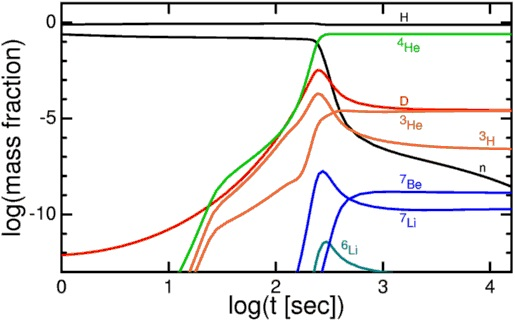
\includegraphics[width=.9\textwidth]{./BBN.jpg}
\caption{Borrowed straight from Ned Wright's tutorial.}
\label{fig:1}
\end{figure}
\section{}
At temperatures above $3\times 10^9 K$ nucleosynthesis cannot occur because all the particles and anti-particles are in thermal equilibrium. The quarks are still forming nucleons so the formation of elements is
impossible.
\newline
The deuterium bottleneck is the fact that deuterium is needed for the formation of helium however due to its low binding energy it is rapidly destroyed by photons at temperatures above $10^9 K$.
\newline
Prior to nucleosynthesis protons and neutrons are in equilibrium with their anti-particles and photons. During nucleosynthesis the neutron/proton ratio was governed by the fact that the neutron has a slightly 
higher rest mass than the proton, and also through weak interactions.
\newline
Helium-4 does not occur through $2n+2p\rightarrow ^{4}He$ because it would involve a highly unlikely 4-body interaction.
\newline
One chain reaction for formation of helium is as follows:
\begin{flalign*}
& p+n\rightarrow^{2}H+\gamma &\\
& ^{2}H+^{2}H\rightarrow ^{3}H+p &\\
& ^{3}H+^{2}H\rightarrow ^{4}He+n
\end{flalign*}
The relative fraction helium is about $25\%$ because it is twice the fraction of neutrons to all nucleons - $2\times0.13=0.26$.
\section{}
I'm guessing here but if neutron decay was 10 times faster then there would be more protons created, and less neutrons, so this would slow helium creation. So, possibly, we would have 10 times less helium that at present.
\section{}
$\Omega_{baryons}$ is the fractional amount of protons and neutrons in the universe. Big Bang nucleosynthesis calculations provide a value of $\Omega_{baryons}$ by first calculating a value $^4He$, and then using this
to calculate values for $D$, $^3He$ and $^7Li$ and finally, using these values, to determine $\Omega_{baryons}$ in the early universe. Measurements from stars and other astronomical objects provide details as to where
the baryons are in the present day.
\section{}
It is hard to directly measure all present day baryons because most baryons seem to be in the form of very hot ionised gas. This is very difficult to detect directly.
%\begin{thebibliography}{1}
%\end{thebibliography}
\end{document} 